\documentclass{article}
\usepackage{hyperref}
\usepackage{graphicx} % Required for inserting images
\usepackage{tabularx}
\usepackage{ltablex}
\usepackage{placeins}
\usepackage[a4paper, total={6in, 8in}]{geometry}

\title{Plan}
\author{Automatic Project Detection And Tooling For Devs}
\date{}

\begin{document}
\maketitle

\section{Full work breakdown}

The work breakdown structure covers all the required functionality in the MVP through three milestones, each addressing core parts of the Model, Persistence, and View layers. It also contains tasks for unit testing to ensure that the program is safe to use.

\subsection*{Milestone 1 - Base Implementation (Due: 2024-11-10)}
\begin{itemize}
    \item Model Layer:
        \begin{itemize}
            \item Implement base classes\@: Argument that represents an argument of a script, ArgumentVisitor that collects the arguments, FileInfo that contains all the data about a script.
            \item Implement must-have functionalities in the Model class: program findig, program running, IO operations.
        \end{itemize}
    \item Persistence Layer:
        \begin{itemize}
            \item Implement IDataAccess interface and DataAccess class to be able to save and load configuration data.
        \end{itemize}
    \item Testing:
        \begin{itemize}
            \item Define and implement unit tests for all classes and functions in Model and Persistence layers.
        \end{itemize}
\end{itemize}

\subsection*{Milestone 2 - View Implementation (Due: 2024-11-30)}
\begin{itemize}
    \item View Layer:
        \begin{itemize}
            \item Implement all the widgets that are needed for each screen\@: text labels, buttons, combo boxes.
            \item Implement all required screens to create the UI\@: RunnerScreen to be able to run the scripts, RunnableConfigScreen to be able to configure the scripts, ShowRunnablesScreen to be able to list all the scripts.
        \end{itemize}
    \item Core Execution:
        \begin{itemize}
            \item Implement main.py to integrate all screens and core functionality.
        \end{itemize}
\end{itemize}

\subsection*{Milestone 3 - Enhanced Functionality and Testing (Due: 2024-12-14)}
\begin{itemize}
    \item Model and View Layers:
        \begin{itemize}
            \item Implement search functionality in both Model and View.
            \item Implement filtering for main runnables.
        \end{itemize}
    \item Testing:
        \begin{itemize}
            \item Develop a comprehensive runner for all test cases.
        \end{itemize}
\end{itemize}

\section{Tasks}

We defined the tasks to be easy to understand and small enough to be done within a few days. The tasks must meet some criteria before getting accepted and merged into the solution:

\begin{itemize}
    \item Unit tests must be written and passed for each new class/function.
    \item UI components must be validated for usability and performance.
    \item Core integrations should function without errors.
    \item Each class, interface, function etc. must have a Python docstring documentation.
\end{itemize}

The full task list is given in Task assignment (section \ref{taskassignment}).

\section{Structure of tasks}

Tasks are structured to reflect dependencies and flow between components:

\begin{itemize}
    \item Milestone 1 tasks are foundational for Model and Persistence layers.
    \item Milestone 2 builds upon Milestone 1, focusing on the View layer.
    \item Milestone 3 completes advanced features and ensures all functionality is tested.
\end{itemize}

\newpage

\section{Task assignment}
\label{taskassignment}

The following table shows task assignments for each developer to ensure accountability.

\subsection{Milestone 1}

\begin{tabularx}{\textwidth} { 
    | >{\raggedright\arraybackslash}X 
    | >{\centering\arraybackslash}X
    | >{\centering\arraybackslash}X | }
    \hline
    \textbf{Task} & \textbf{Developer} & \textbf{Due Date} \\
    \hline
    Implement Argument class in Model layer & Zsófia Laczkó & 2024-10-30 \\
    \hline
    Implement ArgumentVisitor class in Model layer & Benedek Csüllög & 2024-10-30 \\
    \hline
    Implement FileInfo class in Model layer & Borbála Merth & 2024-10-30 \\
    \hline
    Implement IDataAccess interface in Persistence layer & Dániel Gergely & 2024-10-30 \\
    \hline
    Implement DataAccess class inheriting IDataAccess in Persistence layer & Dániel Gergely & 2024-10-30 \\
    \hline
    Implement Model class's base structure in Model layer & Márton Petes & 2024-11-05 \\
    \hline
    Implement Model class's program finding and executable runner functions in Model layer & Zsófia Laczkó & 2024-11-10 \\
    \hline
    Implement Model class's IO operations in Model layer & Márton Petes & 2024-11-10 \\
    \hline
    Define unit tests for Argument class in Tests layer & Borbála Merth & 2024-11-10 \\
    \hline
    Define unit tests for ArgumentVisitor class in Tests layer & Benedek Csüllög & 2024-11-10 \\
    \hline
    Define unit tests for FileInfo class in Tests layer & Borbála Merth & 2024-11-10 \\
    \hline
    Define unit tests for Model class in Tests layer & Márton Petes & 2024-11-10 \\
    \hline
    Define unit tests for DataAccess class in Tests layer & Dániel Gergely & 2024-11-10 \\
    \hline
\end{tabularx}

\newpage

\subsection{Milestone 2}

\begin{tabularx}{\textwidth} { 
    | >{\raggedright\arraybackslash}X 
    | >{\centering\arraybackslash}X
    | >{\centering\arraybackslash}X | }
    \hline
    \textbf{Task} & \textbf{Developer} & \textbf{Due Date} \\
    \hline
    Implement TitleTextLabel widget & Borbála Merth & 2024-11-20 \\
    \hline
    Implement NormalTextLineEdit widget & Borbála Merth & 2024-11-20 \\
    \hline
    Implement NormalTextComboBox widget & Borbála Merth & 2024-11-20 \\
    \hline
    Implement NormalTextLabel widget & Zsófia Laczkó & 2024-11-20 \\
    \hline
    Implement NormalTextButton widget & Benedek Csüllög & 2024-11-20 \\
    \hline
    Implement ComboBox widget in RunnableConfigScreen & TBD & 2024-11-20 \\
    \hline
    Implement RunnableConfigScreen's base structure & Zsófia Laczkó & 2024-11-20 \\
    \hline
    Implement RunnableConfigScreen's string operations & TBD & 2024-11-29 \\
    \hline
    Implement RunnableConfigScreen's input field addition & TBD & 2024-11-29 \\
    \hline
    Implement RunnableConfigScreen's equip button and its functionality & TBD & 2024-11-29 \\
    \hline
    Implement ShowRunnablesScreen's base structure & Dániel Gergely & 2024-11-29 \\
    \hline
    Implement RunnerScreen & Zsófia Laczkó & 2024-11-29 \\
    \hline
    Implement main.py that integrates all the views & Márton Petes & 2024-11-30 \\
    \hline
\end{tabularx}

\newpage

\subsection{Milestone 3}

\begin{tabularx}{\textwidth} { 
    | >{\raggedright\arraybackslash}X 
    | >{\centering\arraybackslash}X
    | >{\centering\arraybackslash}X | }
    \hline
    \textbf{Task} & \textbf{Developer} & \textbf{Due Date} \\
    \hline
    Implement ShowRunnablesScreen's search field & TBD & 2024-12-14 \\
    \hline
    Implement search functionality in Model class & TBD & 2024-12-14 \\
    \hline
    Implement ShowRunnablesScreen's main indications & TBD & 2024-12-14 \\
    \hline
    Implement filtering for main runnables in Model class & TBD & 2024-12-14 \\
    \hline
    Implement filtering for main runnables & TBD & 2024-12-14 \\
    \hline
    Develop test runner & TBD & 2024-12-14 \\
    \hline
    Implement some test runnables & Benedek Csüllög, Márton Petes, Zsófia Laczkó, Dániel Gergely, Borbála Merth & 2024-12-14 \\
    \hline
\end{tabularx}

\section{Time management}

The timeline aligns with each milestone's due date, ensuring the project is completed on schedule:

\begin{itemize}
    \item Milestone 1: Complete by 2024-11-10.
    \item Milestone 2: Complete by 2024-11-30.
    \item Milestone 3: Complete by 2024-12-14.
    \item Sufficient time is allocated for testing and integration after each milestone.
\end{itemize}

\newpage
\section{Architecture}

\subsection{Software components}

The program is built on three main layers, each representing a namespace. These are:

\begin{itemize}
    \item Model: handles the business logic. Finds runnables, and collects its details. Executes the runnables.
    \item Persistence: handles the IO operations. Saves and loads user preferences and other information that is needed for better usability.
    \item View: stands for the user interface.
\end{itemize}

The following image shows the structure of the 3 layer, and all files in the layers. 

\begin{figure}[h]
    \centering
    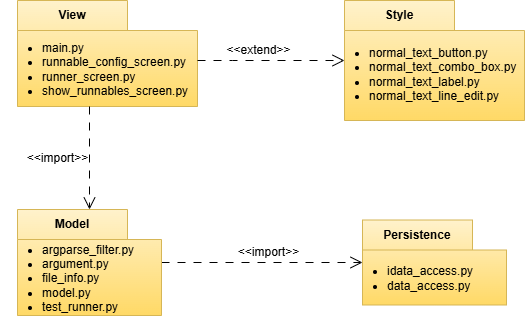
\includegraphics[width=1\linewidth]{img/package_diagram.drawio.png}
    \caption{UML package diagram}
    \label{fig:enter-label}
\end{figure}

The UML class diagram of Model and Persistence layers shows the structure of each object and the relations between them.

\begin{figure}[h]
    \centering
    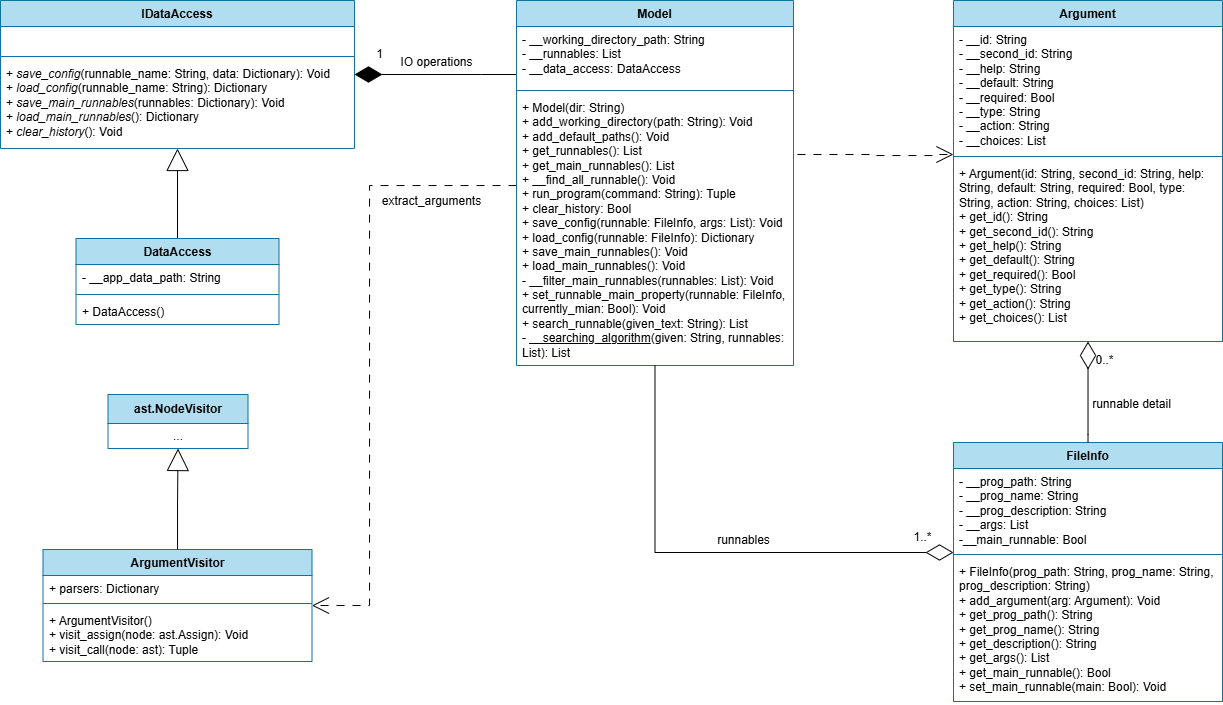
\includegraphics[width=1\linewidth]{img/class_diagram_model_persistence.drawio.png}
    \caption{UML class diagram of Model and Persistence layers}
    \label{fig:enter-label}
\end{figure}

The UML class diagram of View layer shows the structure of each object and the relations between them.

\begin{figure}[h]
    \centering
    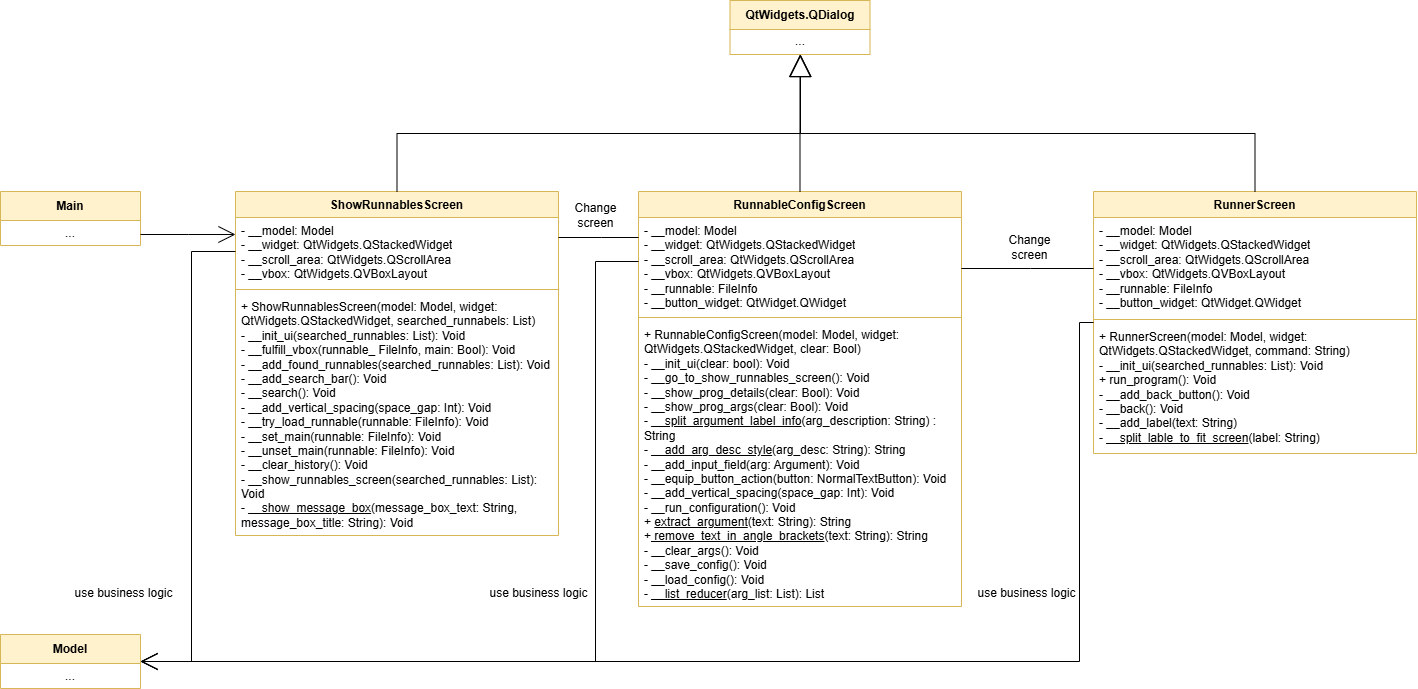
\includegraphics[width=1\linewidth]{img/class_diagram_view.drawio.png}
    \caption{UML class diagram of View layer}
    \label{fig:enter-label}
\end{figure}

The View has 3 screens.

\begin{itemize}
    \item The first one shows all the executables. An executable can be reached with a button. Every executable can be pinned as favourite. The screen also contains a search bar and a clear history button.
    \item The second screen shows an executable all information. Lists all the arguments and offers an opportunity to give a value to it. The user can also run the program here.
    \item The third and last screen shows the output messages, logs or errors for the user, after a program execution.
\end{itemize}

The screens' wire frame plan can be seen below.

\begin{figure}[h]
    \centering
    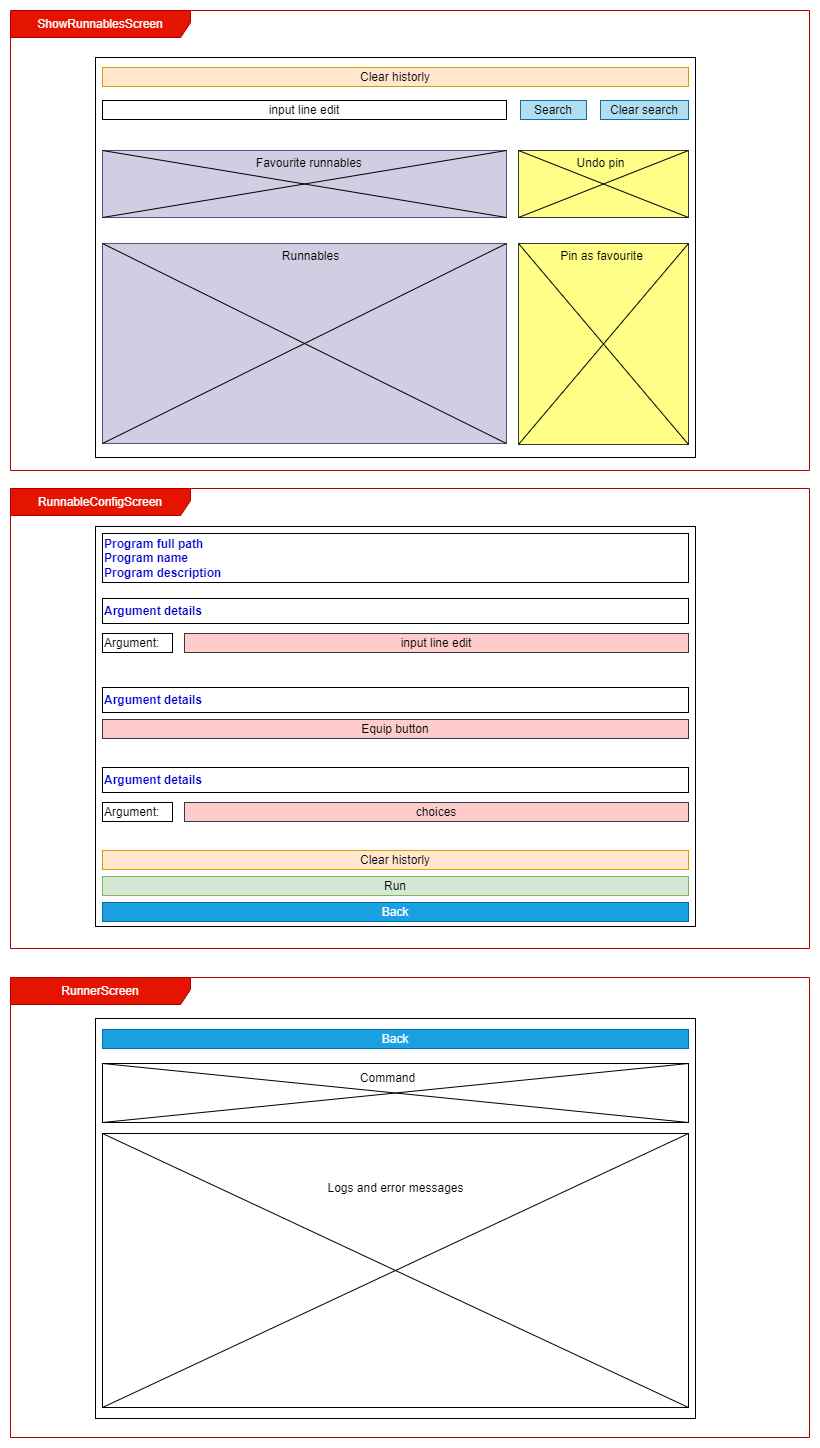
\includegraphics[width=1\linewidth]{img/wire_frame_plan.drawio.png}
    \caption{Screens' wire frame plan}
    \label{fig:enter-label}
\end{figure}

\newpage

\subsection{Software installation}

To install the software, follow these steps:

\begin{enumerate}
    \item Clone the repository\@: \texttt{git clone <repo\_url>}.
    \item Install dependencies\@: Run \texttt{npm install} (for Node.js environment)\\
                                  or \texttt{pip install -r requirements.txt} (for Python).
    \item Start the application\@: \texttt{npm start} or \texttt{python app.py}.
\end{enumerate}

\subsection{Software requirements}

The following tools and environments are required:

\begin{itemize}
    \item Operating System\@: Windows/Linux/MacOS
    \item Programming Language\@: Node.js or Python (v3.8+)
    \item Additional dependencies\@: Docker, PostgreSQL (if applicable)
    \item Disk space\@: At least 500MB of free space
    \item RAM\@: 4GB minimum (recommended 8GB for better performance)
\end{itemize}

\end{document}